\documentclass[oneside]{book}
\usepackage[utf8]{inputenc}
\usepackage{amsmath}
\usepackage{siunitx}
\usepackage{color}
\usepackage{amsfonts}
\usepackage{xcolor}
\usepackage{graphicx}
\usepackage{hyperref}

\usepackage{cleveref}
\crefformat{section}{\S#2#1#3} % see manual of cleveref, section 8.2.1
%\crefformat{chapter}{\S}
%\crefformat{section}{\S}
\crefformat{subsection}{\S#2#1#3}
\crefformat{subsubsection}{\S#2#1#3}


\usepackage{enumitem}

\newcommand{\pd}{\partial}

\title{Fully Self Consistent Simulations of the 1D Fuzzy Dark Matter and Particle System}
\author{Boris Zupancic}
\date{\today}

\begin{document}

\maketitle

\tableofcontents
%---------------------------------------------------------------------------------
% CHAPTER 1: THE SYSTEM

\chapter{The System}

The system is comprised of a Fuzzy Dark Matter (FDM) component, as well as a set of particles, both confined to a 1D box. The FDM and particles share the same gravitational potential, defined by their combined density $\rho$ and Poisson's equation: 
\begin{equation}
\nabla^2 \Phi = 4\pi G \rho    
\label{Poisson}
\end{equation}

The equations of motion (EOM) for FDM and the particles both rely on $\Phi$, but are different, as seen below. Our goal is to numerically integrate these equations of motion in a fully self-consistent manner.

\section{Fuzzy Dark Matter (FDM)}
The EOM for FDM in a periodic box is the Schrodinger-Poisson (SP) system :
\begin{equation}
    \begin{cases}
    i\hbar \frac{\pd \psi}{\pd t} = -\frac{\hbar^2}{2 m_\text{\tiny{FDM}}} \frac{\pd^2 \psi}{\pd x^2} + m_\text{\tiny{FDM}} \Phi \psi 
    \\
    \frac{\pd^2 \Phi}{\pd x^2} = 4\pi G \rho_\text{\tiny{FDM}}= 4\pi G m_\text{\tiny{FDM}} (|\psi|^2 - \langle |\psi|^2 \rangle)
    \end{cases}
    \label{SP}
\end{equation}
where $\hbar$ is the reduced Planck's constant, $m_{FDM}$ is the FDM-particle mass, $\Phi$ is the specific gravitational potential, and $\psi$ is a Schrodinger wave-function. The wave-function $\psi$ specifies the density:
$$\rho_\text{\tiny{FDM}} = m_\text{\tiny{FDM}}|\psi|^2$$
Thus $|\psi|^2$ is interpreted as a number density. Further notice that in Eq(\ref{SP}) the average number density is subtracted off in Poisson's equation. This is due to Gauss' Law requiring that the boundary conditions are null for a periodic box (this "Jean's Swindle" also allows us to solve Eq(\ref{Poisson}) using an FFT method, outlined further down). 

To non-dimensionalize our system Eq(\ref{SP}), we would like length, velocity, time and mass scales, $L_s, v_s,T_s,M_s$, such that
\begin{equation}
    \begin{cases}
    \Phi = v_s^2 \varphi\\
    \psi = L_s^{-3/2} \chi\\
    x = L_s z\\
    t = T_s \tau\\
    m_\text{\tiny{FDM}} = M_s \mu
    \end{cases}
    \label{Substitutions}
\end{equation}
To illustrate, let us fix length and velocity scales $L_s$ and $v_s$, respectively. For example, we may take:
$$L_s = \SI{1}{kpc} $$
$$v_s = \SI{100}{km.s^{-1}}$$
and then define a time scale 
\begin{equation}
T_s  = \frac{L_s}{v_s}
\label{T_scale}
\end{equation}
We may define a mass scale by first setting Newton's constant to unity $G = 1$, then:
\begin{equation}
[G] = M_s^{-1} L_s^3 T_s^{-2} \Rightarrow M_s \equiv \frac{L_s^3}{T_s^2} = v_s^2 L_s 
\label{M_scale}
\end{equation}
We may further define a "fuzziness" parameter 
\begin{equation}
r \equiv \frac{\hbar}{2 m_\text{\tiny{FDM}} v_s L_s}
\label{Fuzziness Param}
\end{equation}
and finally substituting (\ref{Substitutions}) along with $r$ into Eq(\ref{SP}), our dimensionless SP system is:

\begin{equation}
    \begin{cases}
    i\frac{\pd \chi}{\pd \tau} = -r\frac{\pd^2 \chi}{\pd z^2} + \frac{1}{2r}\varphi\chi \\
    
    \frac{\pd^2 \varphi}{\pd z^2} = 4\pi\mu (\chi\chi^* - \langle\chi\chi^*\rangle)
    \end{cases}
    \label{SP-NonDim}
\end{equation}



\section{Particles}
In the particle scenario, the equation of motion is the familiar form of Newton's second law, where for a single particle with position $x$ and mass $m$ in a gravitational potential $U = m\Phi$:
\begin{equation}
    \frac{d^2 x}{d t^2} = -\nabla\Phi = -\frac{\pd}{\pd x}\Phi(x,t)
    \label{ParticlesEOM}
\end{equation}
Substituting the same dimensionless parameters (\ref{Substitutions}) as in the wave scenario into Eq(\ref{ParticlesEOM}):

\begin{equation}
    \frac{d^2 z}{d\tau^2} = -\frac{\pd \varphi}{\pd z}
\end{equation}

The gravitational potential is again given by Poisson's equation, and the particle density is 
\begin{equation}
\rho_\text{part} = n \cdot m_{\text{part}}
\label{Particle density}
\end{equation}

where $n$ is the volumetric/surface/linear number density and $m_{\text{part}}$ is the particle mass. We specify how to non-dimensionlize the particle density further down below in \cref{Poisson's Equation for Particles}, when we address the numerical schemes.
    
\section{Together}\label{Together}
Combining the above information, the dimensionless FDM + Particle system looks like:
\begin{equation}
    \begin{cases}
    i\frac{\pd \chi}{\pd \tau} = -r\frac{\pd^2 \chi}{\pd z^2} + \frac{1}{2r}\varphi\chi \\
    
    \frac{d^2 z}{d\tau^2} = -\frac{\pd \varphi}{\pd z}\\
    
    \frac{\pd^2 \varphi}{\pd z^2} = 4\pi \left[{\varrho} - \langle{\varrho}\rangle\right]
    \end{cases}
    \label{FULL-NonDim}
\end{equation}

where we take ${\varrho}$ as specifying the total dimensionless density, given by the addition of FDM density and Particle density:
\begin{equation}
    \varrho \equiv \varrho_\text{\tiny{FDM}} + \varrho_\text{part} 
\end{equation}

where $\varrho_\text{\tiny{FDM}} = m_\text{\tiny{FDM}}|\chi|^2$, and $\varrho_\text{part}$ is not defined until later, in \cref{Poisson's Equation for Particles}.
%------------------------------------------------------------------------------
% CHAPTER 2: NUMERICAL SCHEMES
\chapter{1D Numerical Schemes}

\section{Initial Setup}
The system is setup on a grid of $N$ linearly spaced points:
\begin{equation}
    z = [z_0, z_1, z_2, ..., z_{N-1}]
    \label{grid}
\end{equation}
(indexing starts with \texttt{i = 0} in Python3). These values will serve as edges for histogramming positions of particles, and positions at which the density, potential and acceleration fields are defined. The width of the bins is the constant
$$dz = z_{i+1} - z_i$$

The choice of $N$ will determine the accuracy of the FFT Poisson Solver described below; a higher value $N$ will both increase the accuracy, and increase the computational cost. 

In any given simulation, we further define the box width $L$, and apply the boundaries:
\begin{align}
    z_0 &= -L/2 \\ 
    z_{N-1} &= L/2
\end{align}

\subsection{Initial Conditions}
Our goal is to now setup an initial distribution of FDM and/or particles.

To create these initial conditions, a collection of particles is generated from a random gaussian distribution centered at 
$$z_\text{center} = \frac{z_0 -z_{N-1}}{2} $$
The standard deviation of this distribution is up to choice (treated as an input parameter in the simulation outlined in Chapter 3). Each particle is given an initial velocity of zero: $v = 0$. Densities of each time step are later calculated, as outlined below.

In the case of FDM, the initial distribution is generated in a similar way, but as a true, smooth gaussian:
\begin{equation}
    \rho(z,t=0) \equiv \frac{M}{\sqrt{2\pi \varsigma^2_\text{\tiny{FDM}}}}\exp\left(-\frac{z^2}{2 \varsigma^2_\text{\tiny{FDM}}}\right)
\end{equation}
where we have taken M to be the total dimensional mass of the system, and $\varsigma_\text{\tiny{FDM}}$ to be the dimensionless standard deviation of the distribution. This ensures that the density profile is normalized such that:
$$\int_{-L/2}^{L/2} \rho dz  = M$$
From here we can define the initial dimensional wavefunction as the square root of the number density:
\begin{equation}
    \psi = \sqrt{\frac{M/m_\text{\tiny{FDM}}}{\sqrt{2\pi \varsigma^2_\text{\tiny{FDM}}}}\exp\left(-\frac{z^2}{2 \varsigma^2_\text{\tiny{FDM}}}\right)}
\end{equation}
this conserves the equation $\rho_\text{\tiny{FDM}} = m\text{\tiny{FDM}} |\psi|^2$, and following \ref{Substitutions} gives the dimensionless initial wavefunction:
\begin{equation}
    \chi(z,\tau=0) = L^{3/2}\sqrt{\frac{M/m_\text{\tiny{FDM}}}{\sqrt{2\pi \varsigma^2_\text{\tiny{FDM}}}}\exp\left(-\frac{z^2}{2 \varsigma^2_\text{\tiny{FDM}}}\right)}
\end{equation}
\section{Calculating Density}
At any given time step of a simulation, it is necessary to calculate the acceleration field defined on the grid. To do this, density must be calculated first. It is straightforward to calculate the FDM density: $\varrho_\text{\tiny{FDM}} = m_\text{\tiny{FDM}}|\chi|^2$. Calculating particle density amounts to histogramming the positions of particles.

Following Equation (\ref{Particle density}), in our numerical scheme, the particle density in a given bin of length $d L_\text{box}$ will be:

\begin{equation}
\rho_k = \frac{n_k}{d L_\text{box}}\cdot \Sigma
\label{Numerical Particle Density}
\end{equation}
where $n_k$ is the number of particles counted in the $k^\text{th}$ bin, and $\Sigma$ is the mass per unit area defined for each particle. Note here that $\Sigma$ must have the specified dimensions in the 1D scenario, as each particle is really treated as an infinite 2D sheet perpendicular to our grid $z$ (see \cref{Spitzer+BinneyTremaineProblem}). 

To retrieve a non-dimensional measure for density, we must consider again our scales. The values above may be written as:
\begin{equation*}
    \begin{cases}
    d L_\text{box} = L_s dz \\
    \Sigma = \frac{M_s}{L_s^2} \sigma
    \end{cases}
\end{equation*}
where $\sigma$ is a newly defined non-dimensional analogue for the mass (per unit area) of each particle. Note that we choose the grid $z$ in Eq(\ref{grid}) as our bin edges, thus the non-dim bin size is $dz$. Substitution of these values into (\ref{Numerical Particle Density}) yields a newly defined (non-dim.) density:
\begin{equation}
    \varrho_k \equiv \frac{L_s^3}{M_s} \rho_k = \frac{n_k}{dz}\sigma
    \label{varrho_part}
\end{equation}
This is $\varrho_k$ is the $\varrho_\text{part}$ talked about in \cref{Together}, just defined in a single bin on the grid Eq(\ref{grid}). 

In practice it is necessary to interpolate the histogrammed values $N_k$ from \textit{between} the grid points $z_0,z_1,...,z_{N-1}$ \textit{onto} the grid points. We do this simply by taking an arbitrary array of length $N$: 
$$\tilde{n} = [\tilde{n}_0, \tilde{n}_1, ..., \tilde{n}_{N-1}]$$
and then for $i \in \{1,2,...,N-2\}$, we let:
$$\tilde{n}_i = \frac{1}{2}(n_{i-1}+n_{i+1})$$
and for $i=0,N-1$:
\begin{align*}
    & \tilde{n}_0 = \frac{1}{2}(n_{N-1} + n_1) \\
    & \tilde{n}_{N-1} = \frac{1}{2}(n_{N-2} + n_0)
\end{align*}
preserving the periodicity of the 1D box. We then re-assign $\forall k \in \{0,...,N-1\}$:
$$n_k \leftarrow \tilde{n}_k $$

\subsection{Poisson's Equation for Particles}\label{Poisson's Equation for Particles}
Now that we have covered how dimensionless particle density is calculated, we can non-dimensionalize the corresponding Poisson's Equation. In the dimensional case, Poisson's equation in a periodic box always looks like:
\begin{equation*}
    \nabla_x^2 \Phi = 4\pi G (\rho - \langle \rho \rangle) 
\end{equation*}

When we make the substitutions $\Phi = v_s^2 \varphi$ and $\rho_k = \frac{N_k}{dL_{box}}\cdot \Sigma$, we get (in our 1D case):
\begin{equation*}
    \frac{v_s^2}{L_s^2}\frac{\pd^2 \varphi}{\pd z^2} = 4\pi \frac{M_s}{L_s^3} \left( \frac{n_k}{\Delta z}\cdot \sigma - \left\langle \frac{n_k}{\Delta z}\cdot \sigma \right\rangle\right)
\end{equation*}
Which reduces to
\begin{equation}
    \frac{\pd^2 \varphi}{\pd z^2} = 4\pi \sigma \left( \frac{n_k}{\Delta z} - \left\langle \frac{n_k}{\Delta z}\right\rangle\right)
    \label{Particle NonDim Poisson's Equation}
\end{equation}
You could plug this back into Eq(\ref{FULL-NonDim}) to get the clearer picture of the full dimensionless FDM+Particle system.

\section{Calculating Potential}\label{Poisson Solver}
The second main ingredient in evolving the system is knowing the gravitational potential $\Phi$, or in the dimensionless case, $\varphi$. We must solve for $\varphi$ from Poisson's Equation corresponding to FDM+Particles, seen in Eq(5), and we do so using a Fast-Fourier-Transform (FFT) method. The basic idea is that applying the Discrete-Discrete Fourier Transform (since we're in a periodic box with a discrete signal/sequence) on Poisson's equation yields:
\begin{equation*}
    \frac{\pd^2}{\pd z^2}\left(\sum_{n=0}^{N-1} \hat{\varphi}(k_n) e^{i k_n z}\right) = 4 \pi \left(\sum_{n=0}^{N-1} \hat{\varrho}(k_n) e^{i k_n z} - \langle\varrho\rangle\right)
\end{equation*}

where $k_n \equiv 2\pi n / L$, $L$ being the length of the box. Notice that $\langle\varrho\rangle = \hat{\varrho}(k_0)$, so that from the above equation we get:
\begin{equation*}
    \begin{cases}
    -k_n^2 \hat{\varphi}(k_n) = 4 \pi \hat{\varrho}(k_n) \text{, $\forall n \in \mathbb{N}$} \\
    0\cdot \hat{\varphi}(0) = 0
    \end{cases}
\end{equation*}
yielding Poisson's equation fully solvable on our 1D mesh by simply applying an FFT to the density and applying an IFFT to the Fourier Coefficients of the potential, defined by:
\begin{equation*}
    \begin{cases}
    \hat{\varphi}(k_n) = - \frac{4 \pi}{k_n^2} \cdot \hat{\varrho}(k_n) \text{, $\forall n \in \mathbb{N}$} \\
    \hat{\varphi}(0) = 0
    \end{cases}
\end{equation*}

\section{Phase Space Distributions}

{\color{red}
[\textbf{Check This}]}

One of the visual tools we'd like to generate in our simulations is the phase space distribution of not just the particles, but the phase space representation of the FDM wavefunction $\chi$ as well.

In our codes, each particle is as instance of a Python class called \texttt{star}, with attributes of mass, position, and velocity. Thus creating a phase space plot simply means creating a scatter plot of each particles phase space position $(z_\text{star},v_\text{star})$ in $\mathbb{R}^2$.

For creating a phase space representation of the FDM component, we turn to a windowed-FFT (or "Short-time Fourier Transform") similar to the Husimi representation. We get the phase space density by convolving, inside an FFT, the wavefunction with a Guassian window of width $\eta$ centered at a position $z$
\begin{equation}
    f(z,k,\tau) \equiv \sum_{m = 0}^{N-1} \left[e^{imk/N}\exp\left({-\frac{(z-\tilde{z})^2}{2\eta^2}}\right)\chi(\tilde{z,\tau})\right]
    \label{PhaseSpace FDM}
\end{equation}
where $k = 2\pi n$ is the wavenumber in the FFT, ranging in $n\in\{0,...,N-1\}$. In NumPy, which we use in our code, this sign convention requires us to use \texttt{numpy.ifft}. By convention, \texttt{numpy.ifft} also divides by $N$, but we don't mind since we re-normalize $f$ right after so that:
\begin{equation}
\int\int f(z,k) dzdk = 1
\end{equation}

\subsection{Choosing the resolution \(\eta\)}\label{Choosing Resolution}
{\color{red}Investigate}


\section{Time Evolution}

The final ingredient in running a fully self-consistent simulation is evolving both the FDM and Particles with the same time-differencing scheme. We use a kick-drift-kick algorithm. Each step in the kick-drift-kick is performed at the same time for FDM and Particles (Kick FDM+Particles, then Drift FDM+Particles, etc). This time-integration scheme is also symplectic (see \cref{KDK Symplectic}).


\subsection{FDM}
For the FDM, we employ a kick-drift-kick algorithm following \cite{Edwards_2018}, \cite{May&Springel_2021}, to solve Eq(\ref{SP-NonDim}):
\begin{align}
    \chi(\tau+\Delta \tau,z) & = \left[\mathcal{T} \circ e^{-i \int_\tau^{\tau+\Delta\tau} \left(-r \pd_z^2 + \frac{1}{2r}\varphi(\tau,z)\right) } \right]\cdot \chi(\tau,z) \\
    &  \approx  \left[ e^{-i\frac{\Delta\tau}{4r}\varphi(\tau+\Delta\tau,z)} \circ e^{ir\Delta\tau \pd_z^2}\circ e^{-i\frac{\Delta\tau}{4r}\varphi(\tau,z)} \right] \cdot \chi(\tau,z)\\
    & = \left[e^{-i\frac{\Delta\tau}{4r}\varphi(\tau+\Delta\tau,z)} \circ \text{FFT}^{-1}\circ e^{ir\Delta\tau k^2}\circ \text{FFT}\circ e^{-i\frac{\Delta\tau}{4r}\varphi(\tau,z)} \right] \cdot \chi(\tau,z)
\end{align}
The "kick-drift-kick" steps are identified as:
\begin{align*}
    & \text{KICK 1:}  \left[ e^{-i\frac{\Delta\tau}{4r}\varphi(\tau,z)}\right] \cdot \chi(\tau,z) \rightarrow \chi'(\tau,z) \\
    &\text{DRIFT:}  \left[\text{ FFT}^{-1}\circ e^{ir\Delta\tau k^2}\circ \text{FFT } \right] \chi'(\tau,z) \rightarrow \chi''(\tau,z) \\
    &\text{Update Potential} \\
    &\text{KICK 2:}  \left[e^{-i\frac{\Delta\tau}{4r}\varphi(\tau+\Delta\tau,z)} \right]\cdot \chi''(\tau,z) \rightarrow \chi(\tau+\Delta\tau,z)
\end{align*}

The "Update Potential" here (and below) means to recalculate the densities $\varrho_\text{\tiny{FDM}}$ and $\varrho_\text{part}$, and then solve Poisson's equation before continuing onto KICK 2.
\subsection{Particles} To evolve the particle system, we again employ a "kick-drift-kick" algorithm based off of that used for the FDM. We solve the particle EOM from Eqs(\ref{FULL-NonDim}), for an individual particle:
\begin{align*}
&\text{KICK 1: } v({\tau+\Delta\tau/2}) = v(\tau) + \frac{\Delta\tau}{2}a(\tau)\\
&\text{DRIFT: } z({\tau+\Delta\tau})+ \Delta\tau v({\tau+\Delta\tau/2})\\
&\text{Update Potential (to get $a({\tau+\Delta\tau/2}) = -\pd_z \varphi({\tau+\Delta\tau/2})$})\\
&\text{KICK 2: } v({\tau+\Delta\tau}) = v({\tau+\Delta\tau/2}) + \frac{\Delta\tau}{2}a({\tau+\Delta\tau/2})\\
\end{align*}

%-------------------------------------------------------------
% SECTION 3: SIMULATIONS
\chapter{Simulations}
So far, the numerical schemes outlined above have been coded in Python3, and a repo is available on GitHub \footnote{\hyperlink{https://github.com/BorisZupancic/FDM_n_Bodies}{BorisZupancic/FDM\_n\_Bodies} on GitHub.}.

In the program, the dimensional scales, as well as $G$,$\hbar$ and the (non-dim.) total Mass $M/M_s$, are all set to unity in arbitrary units (of correct dimension):
\begin{equation*}
    \begin{cases} L_s = 1\\ v_s = 1\\ \end{cases}\Rightarrow \begin{cases}T_s = 1\\ M_s = 1\end{cases} 
\end{equation*}
\begin{equation*}
    \begin{cases}
        G = 1\\
        \hbar = 1\\
        M / M_s = 1\\
    \end{cases}
\end{equation*}
    
Though not previously defined, the total mass of the FDM + Particle system is 
\begin{equation}
    M \equiv M_\text{\tiny{FDM}} + M_\text{part} \\
\end{equation}
where
\begin{align}
    M_\text{\tiny{FDM}} \equiv \int_{-L/2}^{L/2} \rho_\text{\tiny{FDM}} dx & &\text{and}& &
    M_\text{part} \equiv \int_{-L/2}^{L/2} \rho_\text{\tiny{part}} dx
\end{align}

We further define a new expression for the fuzziness parameter $r$ by rearranging:
\begin{align}
    r & \equiv \frac{\hbar}{2m_\text{\tiny{FDM}} v_s L_s}  \\
    & = \frac{1}{4\pi} \left(\frac{h}{m_\text{\tiny{FDM}} \sigma_\text{\tiny{FDM}} R_\text{syst}}\right) \left(\frac{\sigma_\text{\tiny{FDM}}}{v_s}\right) \left(\frac{R_\text{syst}}{L_s}\right) \\
    & = \frac{1}{4\pi} \left(\frac{\sigma_\text{\tiny{FDM}}}{v_s}\right) \left(\frac{R_\text{syst}}{L_s}\right)
    \left(\frac{\lambda_\text{deB}}{R_\text{syst}}\right)
\end{align}

where $\sigma_\text{\tiny{FDM}}$ is the velocity dispersion of the system, $R_\text{syst}$ is the characteristic size of the system,
and $\lambda_\text{deB}$ is the deBroglie wavelength of the FDM "particle". These can be treated as inputs in the simulations.

\section{Inputs}
Simulations take in as input:
\begin{enumerate}
    \item Box Length: L
    \item Percentage of total mass occupied by FDM: \% FDM.
    \item The ratio of velocity dispersion to velocity scale: $\frac{\sigma_\text{\tiny{FDM}}}{v_s}$
    \item The ratio of characteristic size to length scale: $\frac{R_\text{syst}}{L_s}$
    \item The ratio of deBroglie wavelength to characteristic size: $\frac{\lambda_\text{deB}}{R_\text{syst}}$ 
    \item The number of particles (not FDM): Num\_Particles
    \item The standard deviation of the initial distributions for FDM and Particles
\end{enumerate}

From these inputs, all other quantities characteristic to the FDM and particle system(s) can
be determined, and we can run the simulation. From input 2, we know the percentage of mass occupied by particles:
$$\text{\% Particles} = \% 100 - \text{\% FDM}$$

These two percentages give us the mass occupied by each of FDM and particles.

The inputs 3-5 tell us the fuzziness $r$ of the FDM, which gives us the FDM boson mass: $m_\text{\tiny{FDM}}$.
Combining that with the total FDM mass, we can determine the normalization of $\psi$ (or otherwise $\chi$):
$$\int_{-L/2}^{L/2} \psi(x) dx = \frac{M_\text{\tiny{FDM}}}{m_\text{\tiny{FDM}}} \equiv \text{Num\_Bosons}$$
which can be interpreted as the number of FDM bosons present.

In a similar but opposite way, we can determine the particle mass from the total number of particles (input 5):
$$m_\text{part} = \frac{M_\text{part}}{\text{Num\_Particles}}$$

Other parameters like the grid resolution $N$, are set at fixed values in the code.

\subsection{Optional Inputs}
There are other possible/optional inputs in the code, such as: 
\begin{itemize}
    \item Fixing the potential to a quadratic.
    \item Whether to output plots at every time-step or at snapshots.
    \item Diagnostic/Analysis functionalities: 
    \begin{itemize}
        \item Tracking the centroid of the particle distribution.
        \item Tracking the Energies of a few individual particles
        \item Tracking the total Kinetic and Potential Energies of the system.
    \end{itemize}
\end{itemize}

\section{Outputs}
The standard output of the code is the final wavefunction $\chi$ (collected in a csv) and the collection of particles 
(or \texttt{star} class instances), saved in .csv files, as well as plots of the FDM distribution, Particle Distribution, 
their respective phase-space distributions, and a plot of force contributions from FDM and Particles. 

\begin{figure}[h]
    \centering
    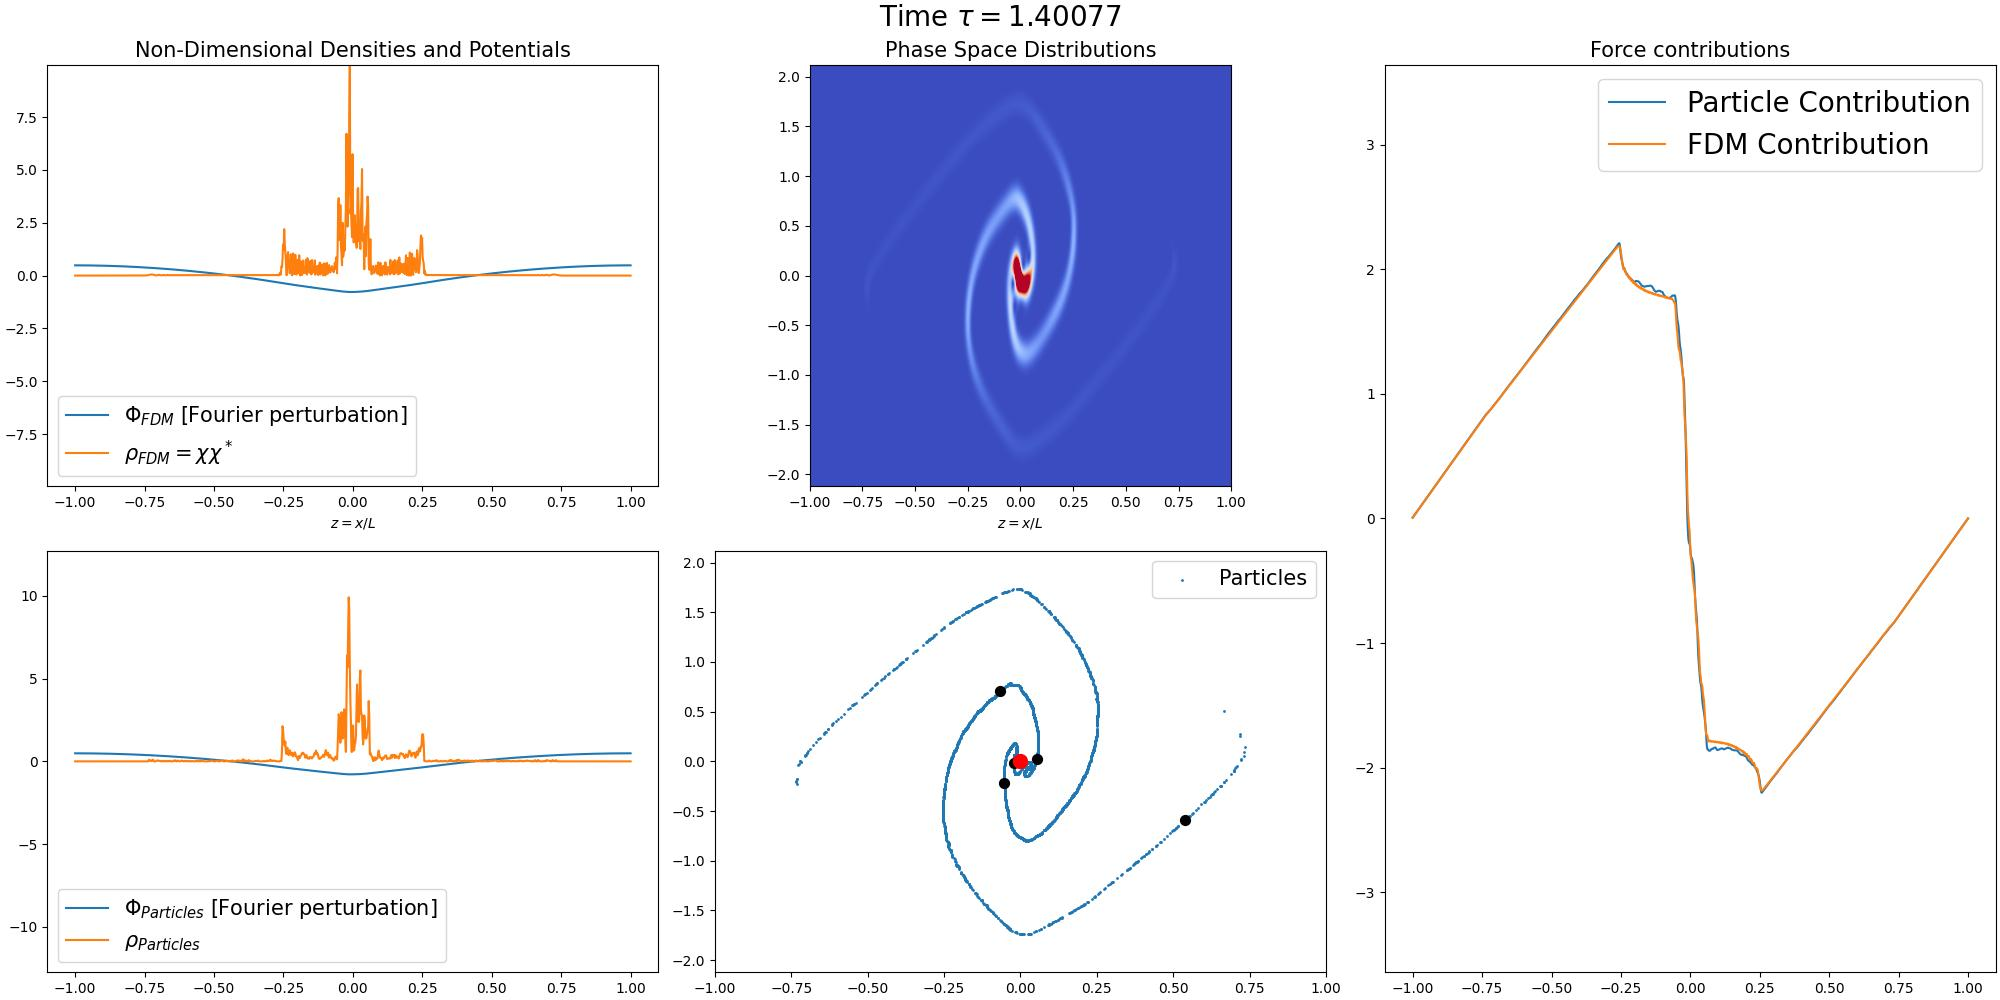
\includegraphics[width=\textwidth]{Images/ToyModelPlot0100.jpg}
    \caption{An example plot from a simulation of a 50\% FDM, 50\% particle system. (Can't remember how many particles, or the specific $r$, or any other input parameters). }
    \label{Example Snapshot}
\end{figure}

The optional diagnostics above are also outputted as arrays and saved in .csv files.

%-------------------------------------------------------------
% Chapter 4: ANALYSIS
\chapter{Analysis + Diagnostics}

\section{Running purely N-Body}
Diagnostics/tests were performed for an array of particle numbers, between 5 and 100000 particles, all generated from a Gaussian distribution of standard deviation 0.1, in a system of total mass $M=1$ (just as described in Chapter 2.)

To illustrate the results of the analysis and diagnostics,  we use the 100000-Body run as the primary example below. We also include an analysis of the convergent behaviour of the system upon increasing the particle number.

\subsection{Energies}
To check that conservation of Energy holds, and to analyse possible oddities in the energy of individual particles over time, we perform several diagnostics tracking Kinetic and Potential Energies.

Kinetic energy for a single particle is calculated simply as:
\begin{equation}
    K = \frac{1}{2}m_\text{part} v^2
\end{equation}
Potential energy for a single particle is calculated by locating the particle's position on the grid by index, then interpolating between grid points to determine what the potential $\Phi$ is at the exact location of the particle, then calculate:
\begin{equation}
    W = m_\text{part}\Phi(x)    
    \label{Potential Energy}
\end{equation}
Now, since the FFT solving method for Poisson's equation, seen in \cref{Poisson Solver}, actually returns
$$\Phi \leftarrow \Phi - \langle\Phi\rangle$$
instead of $\Phi$, we attempt to properly zero the potential by subtracting the maximum value in the box:
$$\Phi \leftarrow \Phi - \sup_{[-L/2,L/2]}(\Phi)$$
and then use this value in the potential energy Eq(\ref{Potential Energy}). 

{\color{red}
We also compute the total potential energy in a given particle system as 
\begin{equation}
    W_\text{tot} = \frac{1}{2} \sum_{i = 1}^{\text{Num\_Particles}} m_\text{part}\Phi(x_i)
    \label{Total Potential Energy}
\end{equation}
(this has been giving me a little trouble, on whether or not to include the factor of 1/2.)}
We of course complete these calculations in our analogous non-dimensional values.

Using these definitions of $K$ and $W$, we track the energies of 5 individual particles, at every time-step. We also track the energies of \textit{all} particles, but only at snapshots in time, defined at indices:
$$i = 99*[0,1,2,4,8,16,32,64]$$
In Figure \ref{5Stars Inidivual} are shown the relevant plots for the 5 individual particles, showing Kinetic,Potential and Total Energies, and in Figure \ref{5Stars Total} are the totals of these energies, along with ``Virial Ratio":
\begin{equation}
    \left|\frac{K}{W}\right|
\end{equation}
\begin{figure}[h]
    \centering
    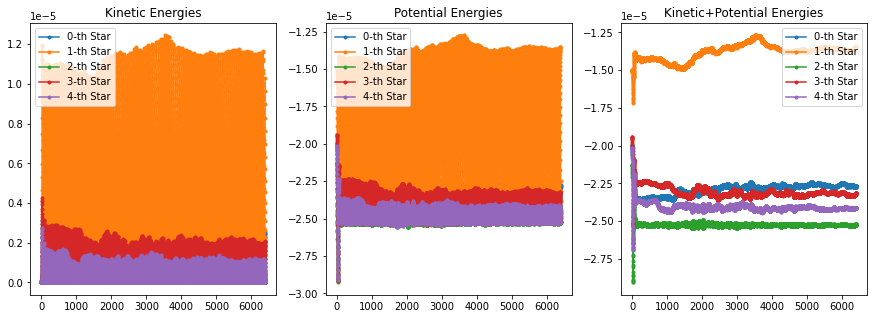
\includegraphics[width=\textwidth]{Images/5Stars_Individual.png}
    \caption{Caption}
    \label{5Stars Inidivual}
\end{figure}

\begin{figure}[h]
    \centering
    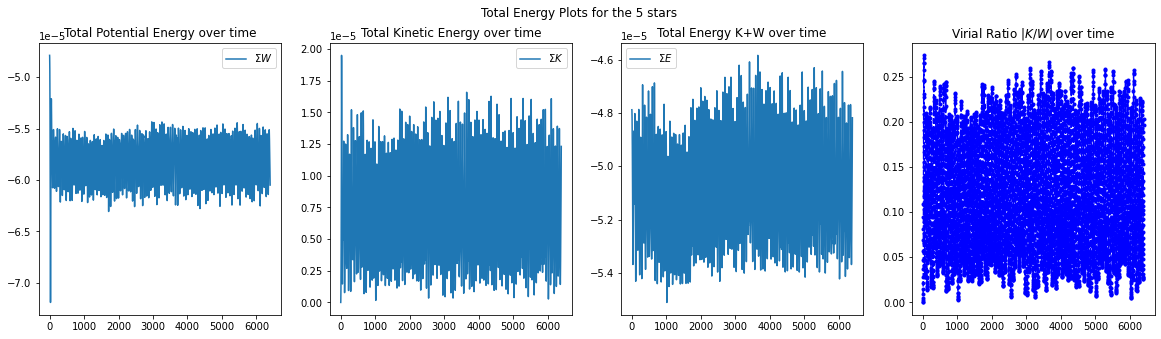
\includegraphics[width=\textwidth]{Images/5Stars_Total.png}
    \caption{Caption}
    \label{5Stars Total}
\end{figure}

Now in Figure \ref{All Total Energies} we see the plot of the same values seen above in  \ref{5Stars Total}, but for every single particle, taken at the snapshot times defined above.
\begin{figure}[h]
    \centering
    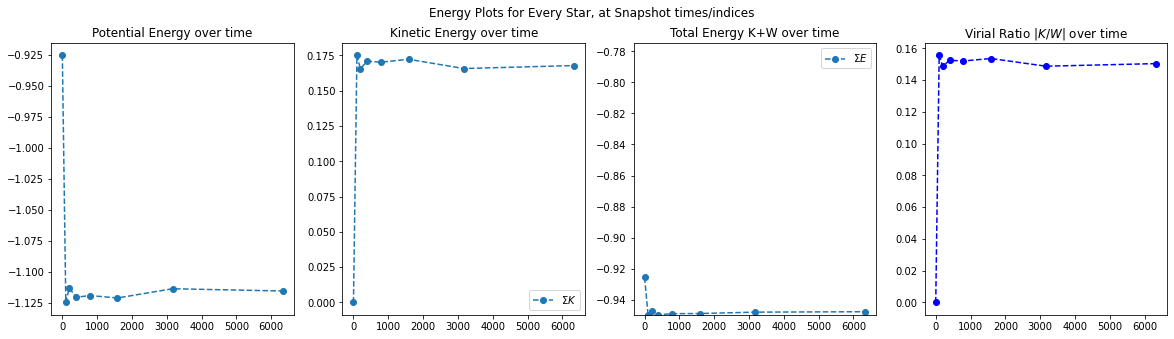
\includegraphics[width=\textwidth]{Images/AllTotal.png}
    \caption{Caption}
    \label{All Total Energies}
\end{figure}

\subsection{Checking the Virial Theorem}
As the simulation goes on, we expect the system to eventually virialize, especially with a large number of particles such as 100000. Visually, this may seem obvious simply by checking that the phase space distribution no longer has any spirals/phase-wrapping, but the Virial theorem specifically states \cite{Binney&Tremaine}:
\begin{align}
    &\text{Tensor:} && \frac{1}{2}\frac{d^2 I_{jk}}{dt^2} = 2K_{jk} + W_{jk} \\
    &\text{Scalar:} && 2K+W=0
\end{align}
As it turns out, in 1D this changes to (see \cref{Spitzer+BinneyTremaineProblem},\cref{1D Virial Theorem}):
\begin{equation}
    K+W=0
    \label{1DVirialEquation}
\end{equation}
and this is what we would like to check.

Note that, while we do wish to check Eq(\ref{1DVirialEquation}), the condition becomes again slightly modified since we have zeroed our gravitational potential energy in an odd way (Eq(\ref{Potential Energy})). 
{\color{red}\textbf{Going to have to check this; since we are in a periodic box, the boundary conditions may not be such that $\Phi \rightarrow 0$ as $x \rightarrow \infty$}.
This means that Eq(\ref{1DVirialEquation}) can actually take the form $K+W = C$, where $C$ is some unknown constant, not to be confused with the constant total Energy.}

\subsection{Centroid Drifting}
An important quantity that should be conserved is the centre of mass of the distribution, so we track this. {\color{red}Currently, it appears to drift over time, and I don't know why}.
\begin{figure}[h]
    \centering
    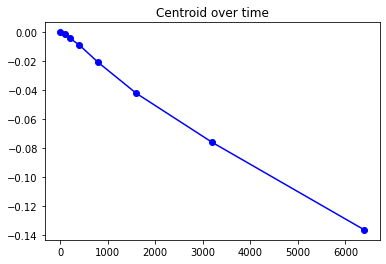
\includegraphics[scale = 0.75]{Images/Centroid.png}
    \caption{Caption}
    \label{Centroid Drift}
\end{figure}
There is also seemingly no pattern in drift direction, or shape, between different instances of the same simulations, and between simulations with different numbers of particles.

\subsection{Virialized Density Profile}
For the amount of time we run the simulation, we expect the system to virialize by the end. We want to see the general form of the density profile in the virialized system.
\begin{figure}[h]
    \centering
    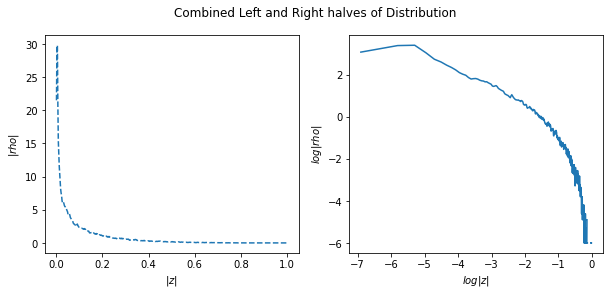
\includegraphics[width = 0.8\textwidth]{Images/DensityProfile.png}
    \caption{Caption}
    \label{Density Profile}
\end{figure}

We manage to curve fit the density profile, with 3 different functions, seen in Figure \ref{Density Curve Fit}.
Most important is the fitting function:
\begin{equation}
    f(z; a_0,a_1,a_2) = \frac{a_0}{|z|^{a_2} (|z|+a_1)^2}
    \label{Fit function}
\end{equation}
where $a_0,a_1,a_2$ are fitting parameters, which resembles a modified NFW profile \cite{NFW1996}.

\begin{figure}[h]
    \centering
    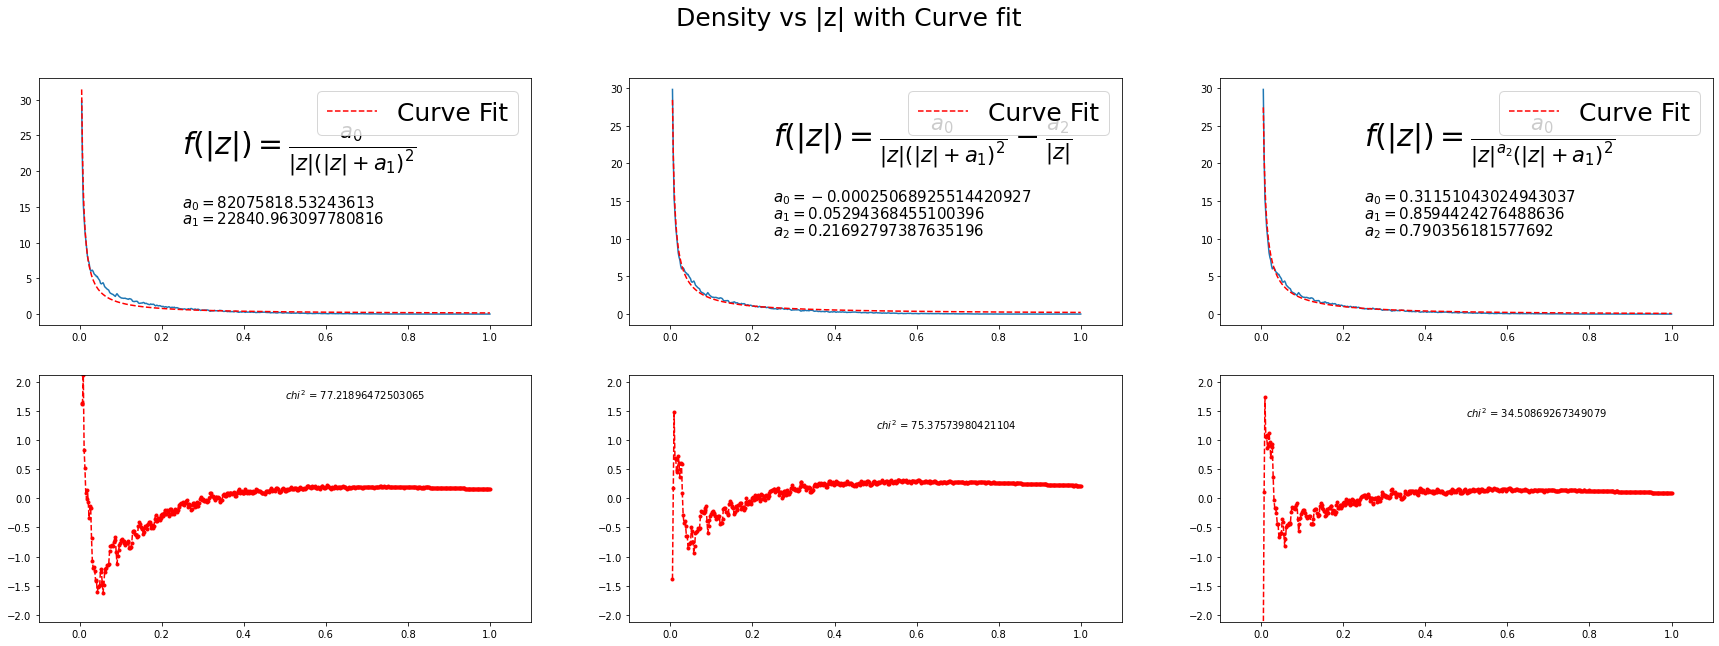
\includegraphics[width = \textwidth]{Images/DensityCurveFit.png}
    \caption{Caption}
    \label{Density Curve Fit}
\end{figure}

\subsection{Virialized Velocity Profile}
Just the same as the density profile approaches a particular distribution, we expect the velocity profile to also approach a particular distribution.
We plot this on the right of Figure \ref{Velocity Profile}, displaying the root-mean-squae velocity $v_\text{rms}$ as a function of radial position $|z|$.
The values are computed by sorting/histogramming the particles by position, the computing the $v_\text{rms}$ in these bins.
A horizontal line through the root-mean-square velocity of \textit{all} particles would represent an isothermal distribution as seen in 
the Spitzer distribution (see problem 4.21 in Binney \& Tremaine \cite{Binney&Tremaine} and \cref{Spitzer+BinneyTremaineProblem}).
\begin{figure}[h]
    \centering
    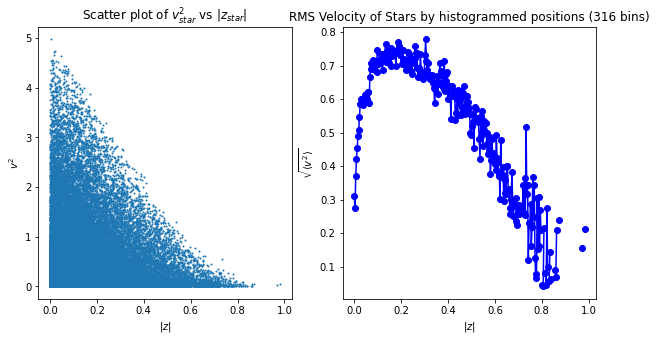
\includegraphics[width = 0.8\textwidth]{Images/VelocityDistribution.png}
    \caption{Caption}
    \label{Velocity Profile}
\end{figure}


\subsection{Convergence of $z_\text{rms}$ and $v_\text{rms}$}
We calculate the root-mean-square position $z_\text{rms}$ and velocity $v_\text{rms}$ at the end of each trial simulation, when the system has virialized.
They should converge as the number of particles increases and the system becomes more ``smooth",
since it approaches a state further resembling that described by the virial equation.
This can be seen in Figure \ref{Z_rms and V_rms Final}.
\begin{figure}[h]
    \centering
    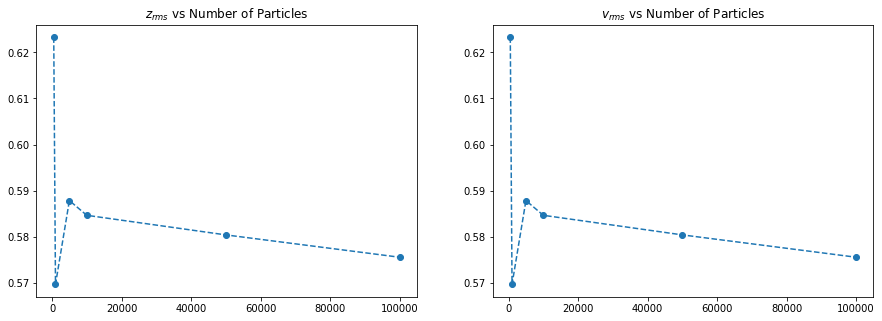
\includegraphics[width=0.8\textwidth]{Images/RMS_Convergence.png}
    \caption{Caption}
    \label{Z_rms and V_rms Final}
\end{figure}


\section{Running purely FDM}

\section{Running Together}



%------------------------------------------
% APPENDIX
\appendix
\chapter{Gravity in 1D}

\section{Spitzer Distribution}\label{Spitzer+BinneyTremaineProblem}

\section{1D Virial Theorem}\label{1D Virial Theorem}

\chapter{Kick-Drift-Kick is Symplectic}\label{KDK Symplectic}


%-----------------------------------------
% BIBLIOGRAPHY
\bibliographystyle{plain} % We choose the "plain" reference style
\bibliography{refs} % Entries are in the refs.bib file

\end{document}


